\chapter{Suppl\texorpdfstring{ementary}{.} material for Chap\texorpdfstring{ter}{.}
\getrefnumber{ch:proteomics}}\label{ch:app-Proteomics}
\chaptermark{Supplementary material for Chapter \getrefnumber{ch:proteomics}}

\begin{figure}[!htbp]
    \centering
    \begin{subfigure}[b]{.5\textwidth}
        \centering 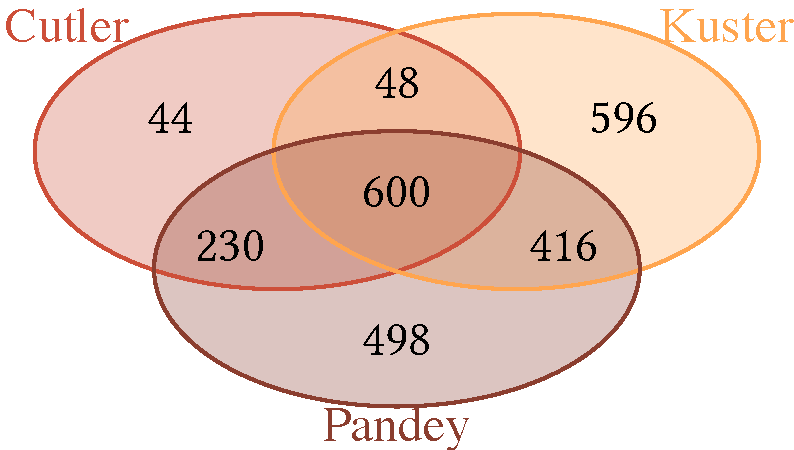
\includegraphics[scale=0.48]{proteomics/VennDiagProtHeart.pdf}
        \caption{Heart}\label{fig:prot3Dheart}
    \end{subfigure}~%
    \begin{subfigure}[b]{.5\textwidth}
        \centering 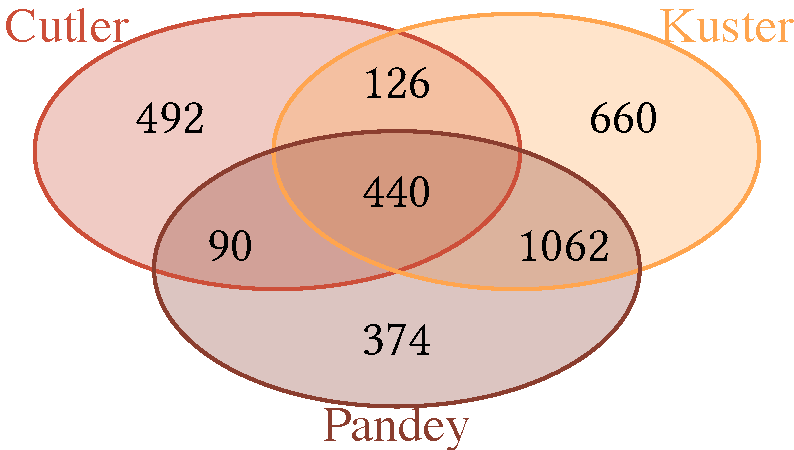
\includegraphics[scale=0.48]{proteomics/VennDiagProtLung.pdf}
        \caption{Lung}\label{fig:prot3Dlung}
    \end{subfigure}

    \begin{subfigure}[b]{.5\textwidth}
        \centering 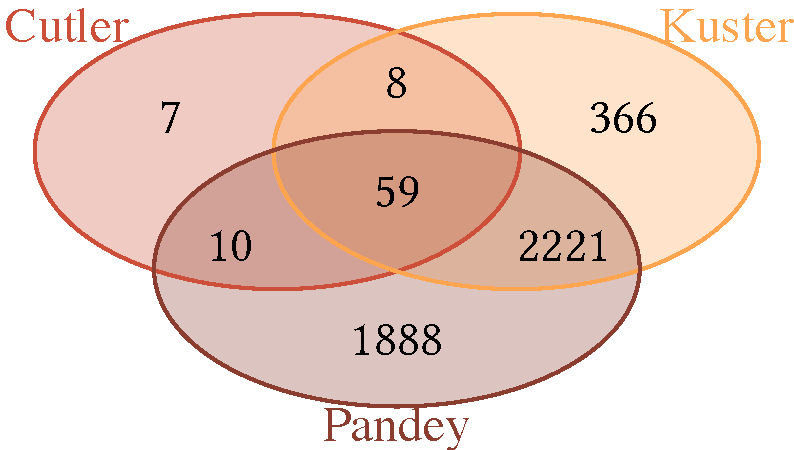
\includegraphics[scale=0.48]{proteomics/VennDiagProtOvary.pdf}
        \caption{Ovary}\label{fig:prot3Dovary}
    \end{subfigure}~%
    \begin{subfigure}[b]{.5\textwidth}
        \centering 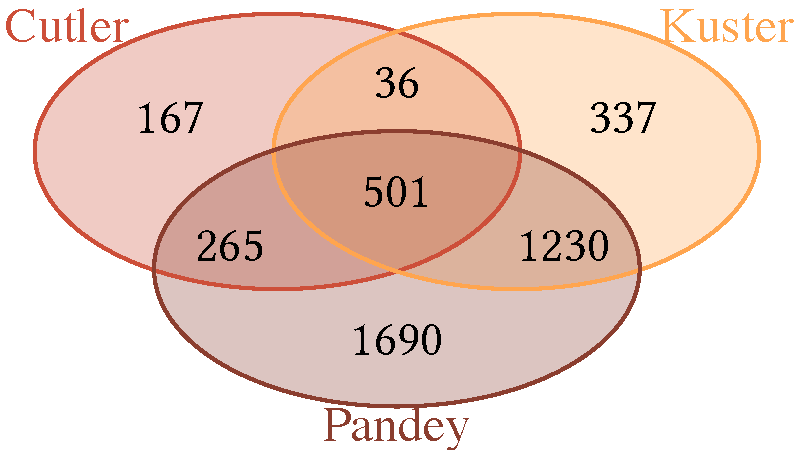
\includegraphics[scale=0.48]{proteomics/VennDiagProtPancreas.pdf}
        \caption{Pancreas}\label{fig:prot3Dpancreas}
    \end{subfigure}
    \caption[Unique and shared proteins across the proteomic studies]%
    {\label{fig:protbkdownT}\textbf{Unique and shared proteins
    across the proteomic studies}}
\end{figure}


\begin{figure}[!htbp]
    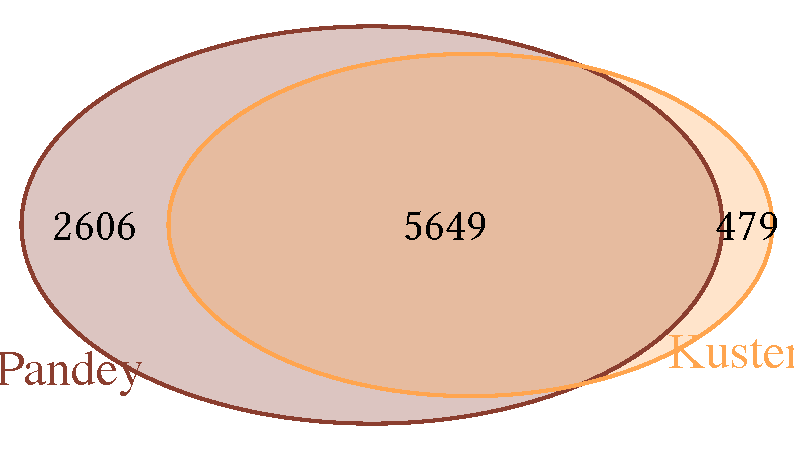
\includegraphics[scale=0.65]{proteomics/VennDiagProtFor14T2D.pdf}\centering
    \caption[Proteins overlap between the common tissues of Pandey and Kuster
    data]{\label{fig:VennDiagProt2D}\textbf{Proteins overlap between the fourteen
    common tissues between Pandey and Kuster proteome data.}}
\end{figure}

\begin{figure}[!htbp]
    \centering
    \begin{subfigure}[b]{.5\textwidth}
        \centering 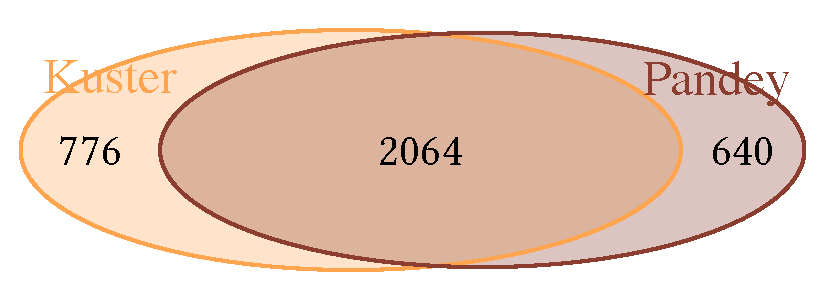
\includegraphics[scale=0.5]{proteomics/VennDiagProtForKusterPandey-Adrenal.pdf}
        \caption{Adrenal}\label{fig:prot3Dadrenal}
    \end{subfigure}~%
    \begin{subfigure}[b]{.5\textwidth}
        \centering 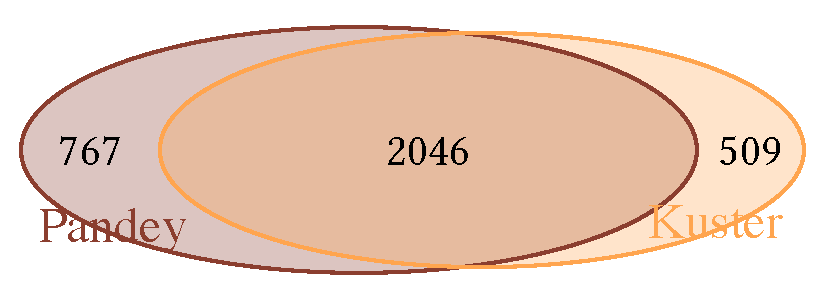
\includegraphics[scale=0.5]{proteomics/VennDiagProtForKusterPandey-Colon.pdf}
        \caption{Colon}\label{fig:prot3Dcolon}
    \end{subfigure}

    \begin{subfigure}[b]{.5\textwidth}
        \centering 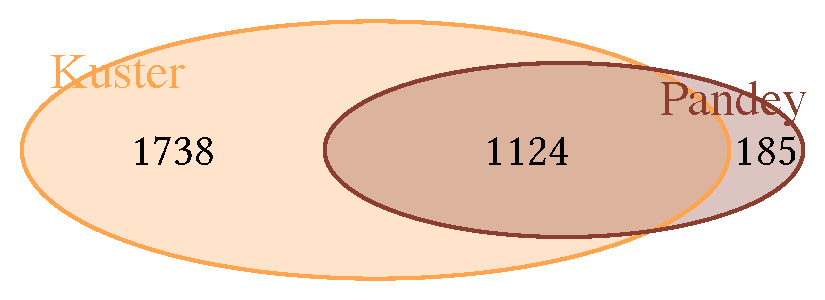
\includegraphics[scale=0.5]{proteomics/VennDiagProtForKusterPandey-Oesophagus.pdf}
        \caption{Oesophagus}\label{fig:prot3Doesophagus}
    \end{subfigure}~%
    \begin{subfigure}[b]{.5\textwidth}
        \centering 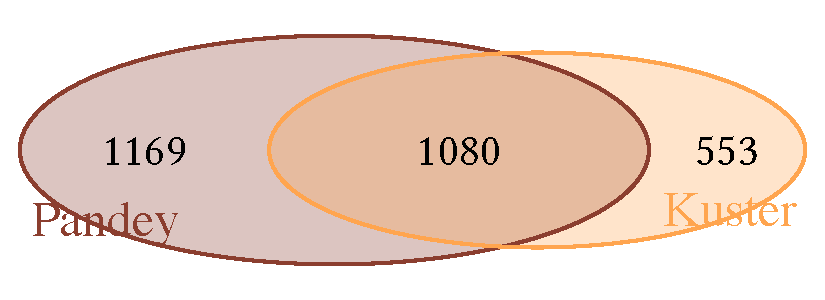
\includegraphics[scale=0.5]{proteomics/VennDiagProtForKusterPandey-Gallbladder.pdf}
        \caption{Gall bladder}\label{fig:prot3Dgallbladder}
    \end{subfigure}

    \begin{subfigure}[b]{.5\textwidth}
        \centering 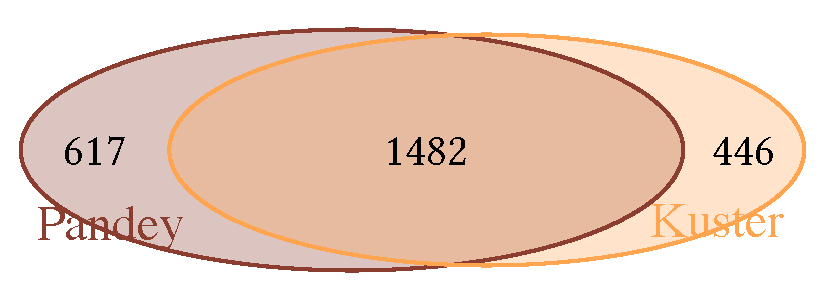
\includegraphics[scale=0.5]{proteomics/VennDiagProtForKusterPandey-Kidney.pdf}
        \caption{Kidney}\label{fig:prot3Dkidney}
    \end{subfigure}~%
    \begin{subfigure}[b]{.5\textwidth}
        \centering 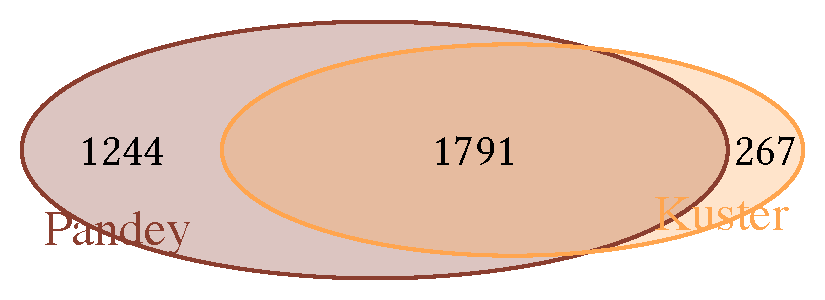
\includegraphics[scale=0.5]{proteomics/VennDiagProtForKusterPandey-Liver.pdf}
        \caption{Liver}\label{fig:prot3Dliver}
    \end{subfigure}

    \begin{subfigure}[b]{.5\textwidth}
        \centering 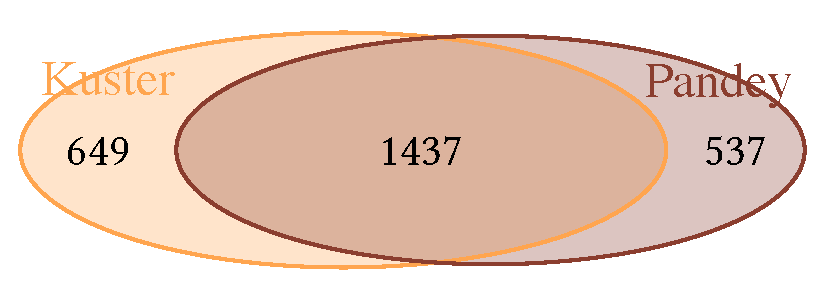
\includegraphics[scale=0.5]{proteomics/VennDiagProtForKusterPandey-Placenta.pdf}
        \caption{Placenta}\label{fig:prot3Dplacenta}
    \end{subfigure}~%
    \begin{subfigure}[b]{.5\textwidth}
        \centering 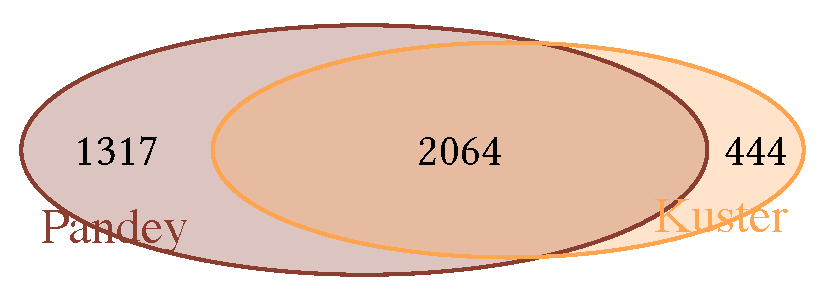
\includegraphics[scale=0.5]{proteomics/VennDiagProtForKusterPandey-Prostate.pdf}
        \caption{Prostate}\label{fig:prot3Dprostate}
    \end{subfigure}

    \begin{subfigure}[b]{.5\textwidth}
        \centering 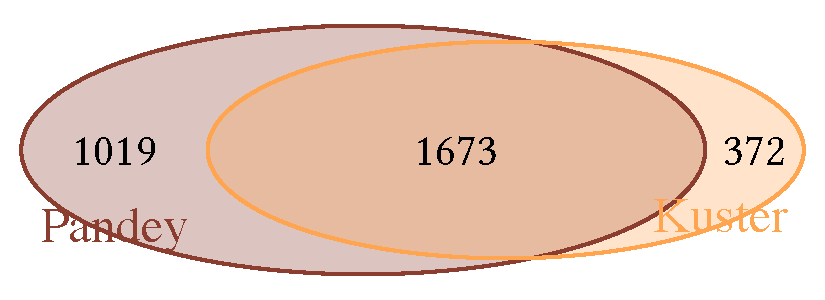
\includegraphics[scale=0.5]{proteomics/VennDiagProtForKusterPandey-Rectum.pdf}
        \caption{Rectum}\label{fig:prot3Drectum}
    \end{subfigure}~%
    \begin{subfigure}[b]{.5\textwidth}
        \centering 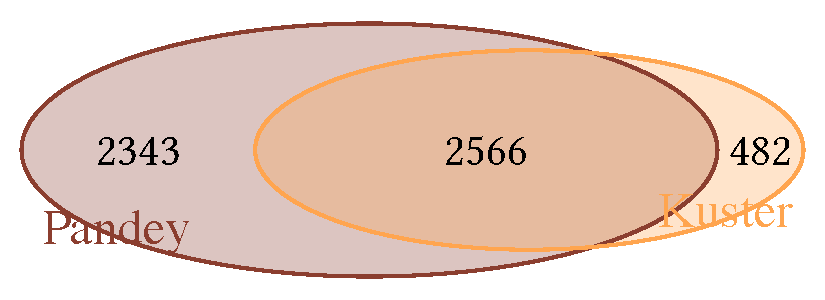
\includegraphics[scale=0.5]{proteomics/VennDiagProtForKusterPandey-Testis.pdf}
        \caption{Testis}\label{fig:prot3Dtestis}
    \end{subfigure}

    \caption[Unique and shared proteins across the other 10 common tissues between Pandey and Kuster proteinseomic studies]%
    {\label{fig:protbkdownT10more}\textbf{Unique and shared proteins
    across the other ten common tissues between Pandey and Kuster proteomic studies}}
\end{figure}


\begin{table}[!htbp]
\centering
\caption{Proteins found in every tissue in all three datasets}\label{tab:ubiProt3D}
\begin{tabular}{ll}
  \toprule
    Ensembl (76) gene ID & Gene symbol \\
  \midrule
  ENSG00000163631 & \gene{ALB} \\
  ENSG00000171403 & \gene{KRT9} \\
  ENSG00000186395 & \gene{KRT10} \\
\bottomrule
\end{tabular}
\end{table}

\begin{table}[!htpb]
    \centering
    \caption{Proteins found in every tissue in Pandey and Kuster datasets}\label{tab:ubiProt2D}
    \begin{tabular}{ll}
        \toprule
        Ensembl (76) ID & Gene symbol \\
        \midrule
        ENSG00000023191 & \gene{RNH1} \\
        ENSG00000044574 & \gene{HSPA5} \\
        ENSG00000067225 & \gene{PKM} \\
        ENSG00000071127 & \gene{WDR1} \\
        ENSG00000074800 & \gene{ENO1} \\
        ENSG00000080824 & \gene{HSP90AA1} \\
        ENSG00000089220 & \gene{PEBP1} \\
        ENSG00000089597 & \gene{GANAB} \\
        ENSG00000092820 & \gene{EZR} \\
        ENSG00000096384 & \gene{HSP90AB1} \\
        ENSG00000100345 & \gene{MYH9} \\
        ENSG00000102144 & \gene{PGK1} \\
        ENSG00000108518 & \gene{PFN1} \\
        ENSG00000108953 & \gene{YWHAE} \\
        ENSG00000111530 & \gene{CAND1} \\
        ENSG00000111640 & \gene{GAPDH} \\
        ENSG00000111669 & \gene{TPI1} \\
        ENSG00000111716 & \gene{LDHB} \\
        ENSG00000117450 & \gene{PRDX1} \\
        ENSG00000130985 & \gene{UBA1} \\
\bottomrule
\end{tabular}%
\begin{tabular}{ll}
    \toprule
    ENSEMBL (76) ID & Gene symbol \\
    \midrule
    ENSG00000134308 & \gene{YWHAQ} \\
    ENSG00000134333 & \gene{LDHA} \\
    ENSG00000140575 & \gene{IQGAP1} \\
    ENSG00000148180 & \gene{GSN} \\
    ENSG00000149925 & \gene{ALDOA} \\
    ENSG00000160752 & \gene{FDPS} \\
    ENSG00000163631 & \gene{ALB} \\
    ENSG00000164924 & \gene{YWHAZ} \\
    ENSG00000165280 & \gene{VCP} \\
    ENSG00000166598 & \gene{HSP90B1} \\
    ENSG00000166794 & \gene{PPIB} \\
    ENSG00000167658 & \gene{EEF2} \\
    ENSG00000170027 & \gene{YWHAG} \\
    ENSG00000170248 & \gene{PDCD6IP} \\
    ENSG00000171403 & \gene{KRT9} \\
    ENSG00000178209 & \gene{PLEC} \\
    ENSG00000179218 & \gene{CALR} \\
    ENSG00000182718 & \gene{ANXA2} \\
    ENSG00000186395 & \gene{KRT10} \\
    ENSG00000204628 & \gene{GNB2L1} \\
   \bottomrule
\end{tabular}
\end{table}

\begin{landscape}
\begin{table}[!htbp]
\centering
\caption{Tissue specific proteins found both in Pandey \etal\ and Kuster \etal\ datasets\label{tab:comTSprot}}
\hspace{-2cm}\begin{tabular}{lll}
\toprule
Tissue & Ensembl (76) ID & Gene symbol \\
\midrule
\adrenal\  & ENSG00000141744 & \gene{PNMT} \\
\adrenal\  & ENSG00000148655 & \gene{C10orf11} \\
\adrenal\  & ENSG00000160882 & \gene{CYP11B1} \\
\adrenal\  & ENSG00000163428 & \gene{LRRC58} \\
\adrenal\  & ENSG00000163626 & \gene{COX18} \\
\kidney\   & ENSG00000074803 & \gene{SLC12A1} \\
\kidney\   & ENSG00000100253 & \gene{MIOX} \\
\kidney\   & ENSG00000112499 & \gene{SLC22A2} \\
\kidney\   & ENSG00000113361 & \gene{CDH6} \\
\kidney\   & ENSG00000148942 & \gene{SLC5A12} \\
\kidney\   & ENSG00000149452 & \gene{SLC22A8} \\
\kidney\   & ENSG00000154025 & \gene{SLC5A10} \\
\kidney\   & ENSG00000158296 & \gene{SLC13A3} \\
\kidney\   & ENSG00000169344 & \gene{UMOD} \\
\kidney\   & ENSG00000170482 & \gene{SLC23A1} \\
\kidney\   & ENSG00000186335 & \gene{SLC36A2} \\
\kidney\   & ENSG00000197901 & \gene{SLC22A6} \\
\liver\    & ENSG00000084734 & \gene{GCKR} \\
\liver\    & ENSG00000100197 & \gene{CYP2D6} \\
\liver\    & ENSG00000135094 & \gene{SDS} \\
\liver\    & ENSG00000172497 & \gene{ACOT12} \\
\liver\    & ENSG00000198650 & \gene{TAT} \\
\pancreas\ & ENSG00000010438 & \gene{PRSS3} \\
\bottomrule
\end{tabular}%
\begin{tabular}{lll}
\toprule
Tissue & Ensembl (76) ID & Gene symbol \\
\midrule
\pancreas\ & ENSG00000114204 & \gene{SERPINI2} \\
\pancreas\ & ENSG00000141086 & \gene{CTRL} \\
\pancreas\ & ENSG00000143954 & \gene{REG3G} \\
\pancreas\ & ENSG00000187021 & \gene{PNLIPRP1} \\
\pancreas\ & ENSG00000215704 & \gene{CELA2B} \\
\pancreas\ & ENSG00000266200 & \gene{PNLIPRP2} \\
\placenta\ & ENSG00000105825 & \gene{TFPI2} \\
\placenta\ & ENSG00000116183 & \gene{PAPPA2} \\
\placenta\ & ENSG00000137868 & \gene{STRA6} \\
\placenta\ & ENSG00000148848 & \gene{ADAM12} \\
\placenta\ & ENSG00000163283 & \gene{ALPP} \\
\placenta\ & ENSG00000172296 & \gene{SPTLC3} \\
\placenta\ & ENSG00000172901 &  \\
\placenta\ & ENSG00000183668 & \gene{PSG9} \\
\placenta\ & ENSG00000243137 & \gene{PSG4} \\
\prostate\ & ENSG00000044524 & \gene{EPHA3} \\
\prostate\ & ENSG00000103710 & \gene{RASL12} \\
\rectum\   & ENSG00000205277 & \gene{MUC12} \\
\testis\   & ENSG00000052841 & \gene{TTC17} \\
\testis\   & ENSG00000109762 & \gene{SNX25} \\
\testis\   & ENSG00000130948 & \gene{HSD17B3} \\
\testis\   & ENSG00000160310 & \gene{PRMT2} \\
& &\\
\bottomrule
\end{tabular}
\end{table}
\end{landscape}

\begin{comment}
\begin{longtable}{@{}cll@{}}%
\caption{Tissue specific proteins found both in Pandey \etal\ and Kuster \etal\ datasets\label{tab:comTSprot}}\\
\toprule
Tissue & Ensembl (76) ID & Gene symbol \\* \midrule
\endfirsthead
\caption[]{Tissue specific proteins found both in Pandey \etal\ and Kuster \etal\ datasets}\\
\toprule
Tissue & Ensembl (76) ID & Gene symbol \\* \midrule
\endhead
%
\bottomrule
\endfoot
%
\endlastfoot
%
\adrenal\  & ENSG00000141744 & \gene{PNMT} \\
\adrenal\  & ENSG00000148655 & \gene{C10orf11} \\
\adrenal\  & ENSG00000160882 & \gene{CYP11B1} \\
\adrenal\  & ENSG00000163428 & \gene{LRRC58} \\
\adrenal\  & ENSG00000163626 & \gene{COX18} \\
\kidney\   & ENSG00000074803 & \gene{SLC12A1} \\
\kidney\   & ENSG00000100253 & \gene{MIOX} \\
\kidney\   & ENSG00000112499 & \gene{SLC22A2} \\
\kidney\   & ENSG00000113361 & \gene{CDH6} \\
\kidney\   & ENSG00000148942 & \gene{SLC5A12} \\
\kidney\   & ENSG00000149452 & \gene{SLC22A8} \\
\kidney\   & ENSG00000154025 & \gene{SLC5A10} \\
\kidney\   & ENSG00000158296 & \gene{SLC13A3} \\
\kidney\   & ENSG00000169344 & \gene{UMOD} \\
\kidney\   & ENSG00000170482 & \gene{SLC23A1} \\
\kidney\   & ENSG00000186335 & \gene{SLC36A2} \\
\kidney\   & ENSG00000197901 & \gene{SLC22A6} \\
\liver\    & ENSG00000084734 & \gene{GCKR} \\
\liver\    & ENSG00000100197 & \gene{CYP2D6} \\
\liver\    & ENSG00000135094 & \gene{SDS} \\
\liver\    & ENSG00000172497 & \gene{ACOT12} \\
\liver\    & ENSG00000198650 & \gene{TAT} \\
\pancreas\ & ENSG00000010438 & \gene{PRSS3} \\
\pancreas\ & ENSG00000114204 & \gene{SERPINI2} \\
\pancreas\ & ENSG00000141086 & \gene{CTRL} \\
\pancreas\ & ENSG00000143954 & \gene{REG3G} \\
\pancreas\ & ENSG00000187021 & \gene{PNLIPRP1} \\
\pancreas\ & ENSG00000215704 & \gene{CELA2B} \\
\pancreas\ & ENSG00000266200 & \gene{PNLIPRP2} \\
\placenta\ & ENSG00000105825 & \gene{TFPI2} \\
\placenta\ & ENSG00000116183 & \gene{PAPPA2} \\
\placenta\ & ENSG00000137868 & \gene{STRA6} \\
\placenta\ & ENSG00000148848 & \gene{ADAM12} \\
\placenta\ & ENSG00000163283 & \gene{ALPP} \\
\placenta\ & ENSG00000172296 & \gene{SPTLC3} \\
\placenta\ & ENSG00000172901 &  \\
\placenta\ & ENSG00000183668 & \gene{PSG9} \\
\placenta\ & ENSG00000243137 & \gene{PSG4} \\
\prostate\ & ENSG00000044524 & \gene{EPHA3} \\
\prostate\ & ENSG00000103710 & \gene{RASL12} \\
\rectum\   & ENSG00000205277 & \gene{MUC12} \\
\testis\   & ENSG00000052841 & \gene{TTC17} \\
\testis\   & ENSG00000109762 & \gene{SNX25} \\
\testis\   & ENSG00000130948 & \gene{HSD17B3} \\
\testis\   & ENSG00000160310 & \gene{PRMT2} \\* \bottomrule
\end{longtable}
\end{comment}
\begin{figure}[!htbp]
    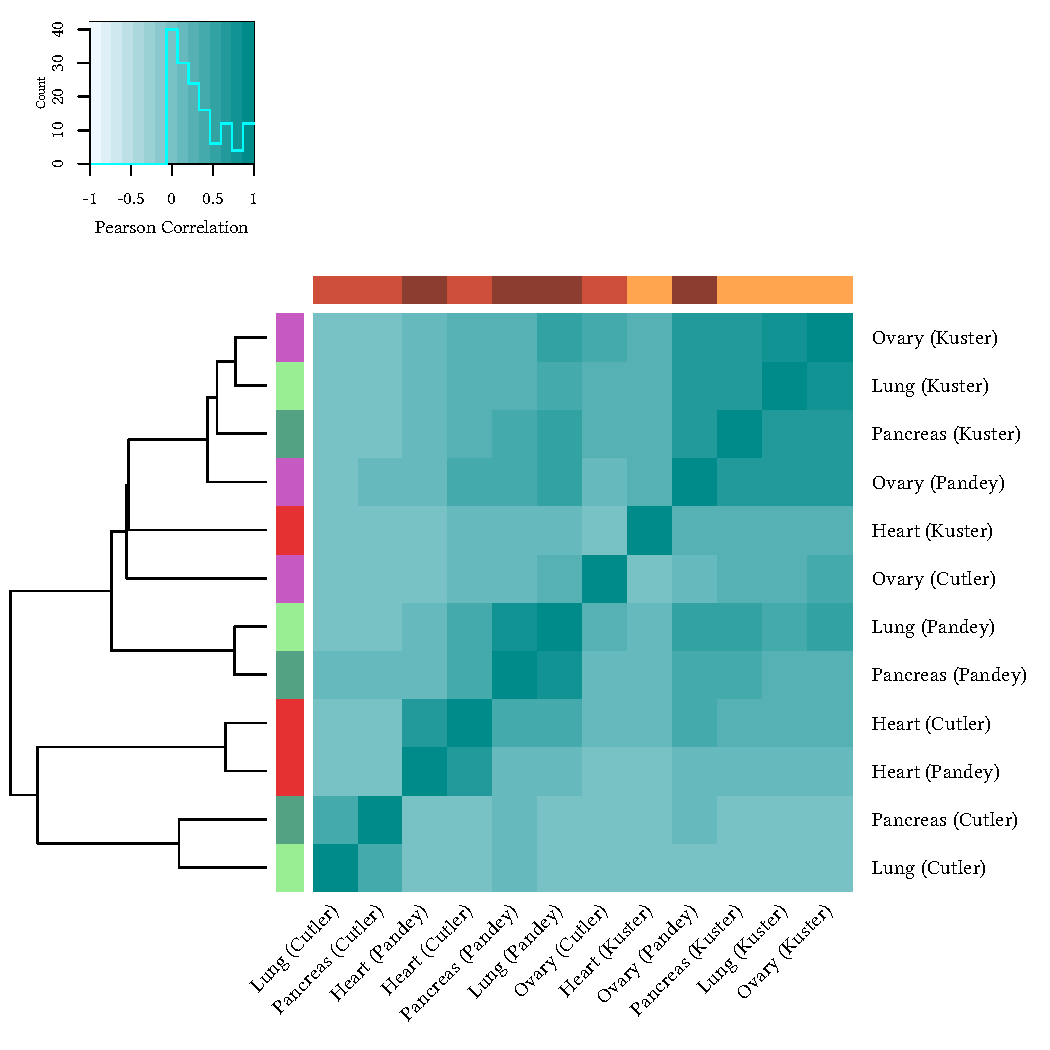
\includegraphics[scale=0.7]{proteomics/heatmap3DproteinPearson.pdf}\centering
    \vspace{-4mm}
    \caption[Heatmap of the 4 common tissues between the three proteome
    datasets (Pearson correlation)]{\label{fig:prot3DheatmapPears}\textbf{Heatmap
    of the four common tissues between the three proteome datasets}
    based on the pairwise \textbf{Pearson correlations} clustering of
    1,384 proteins expression levels.
    See \Cref{fig:prot3Dheatmap} for the heatmap based on Spearman correlation.}
\end{figure}

\begin{figure}[!htpb]
    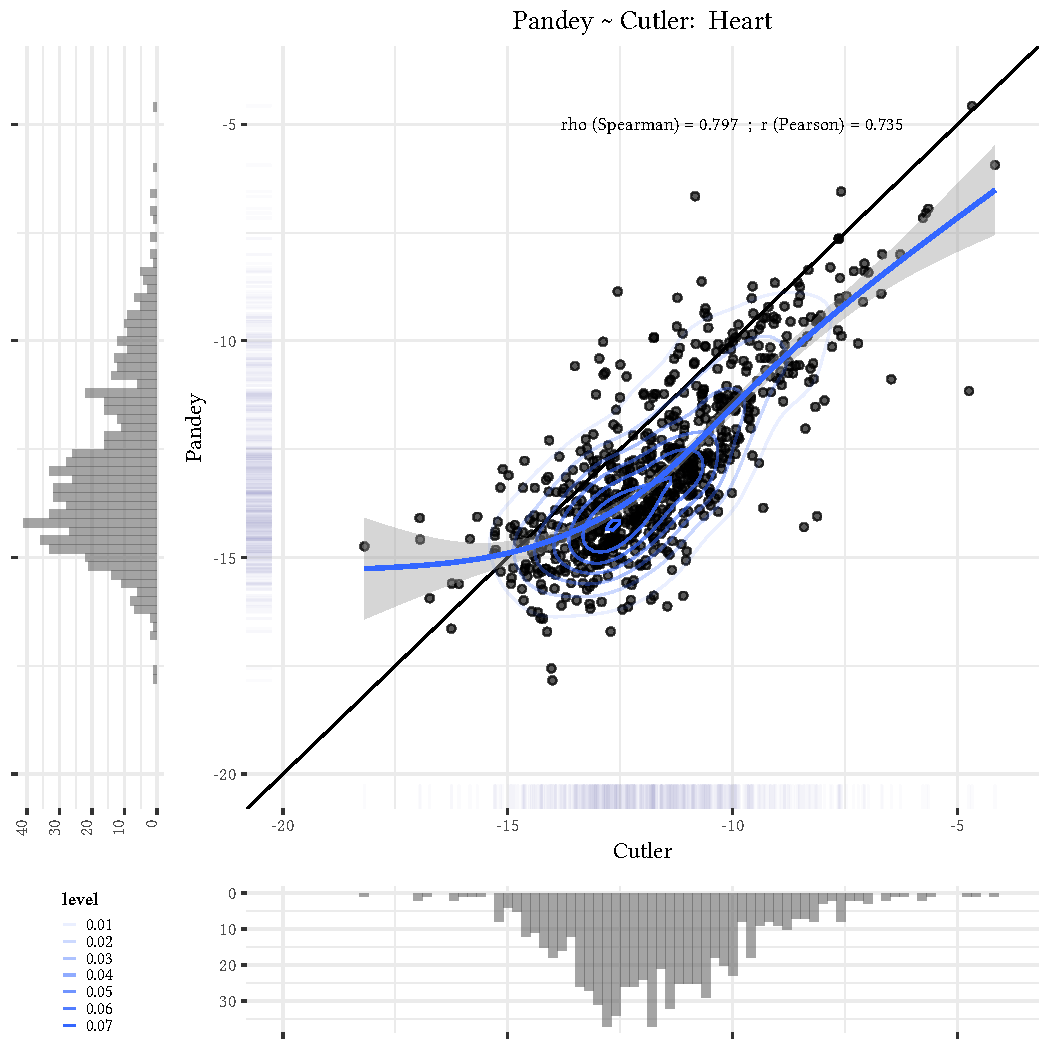
\includegraphics[scale=0.7]{proteomics/scatterplot/3D/heartCutlerPandey.pdf}\centering
    \caption[Heart: Cutler vs Pandey]{\label{fig:scat3DheartCutlerPandey}\textbf{%
    Scatterplot of Heart for Cutler and Pandey data.}
    There is an overall strong correlation between
    the expression of the \heart\ proteins
    between \pandey\ (y-axis) and \cutler\ (x-axis)
    even though the dispersion is quite substantial.
    {\small The black line $y=x$ is only present as a visual reference.}}
\end{figure}

\begin{figure}[!htpb]
    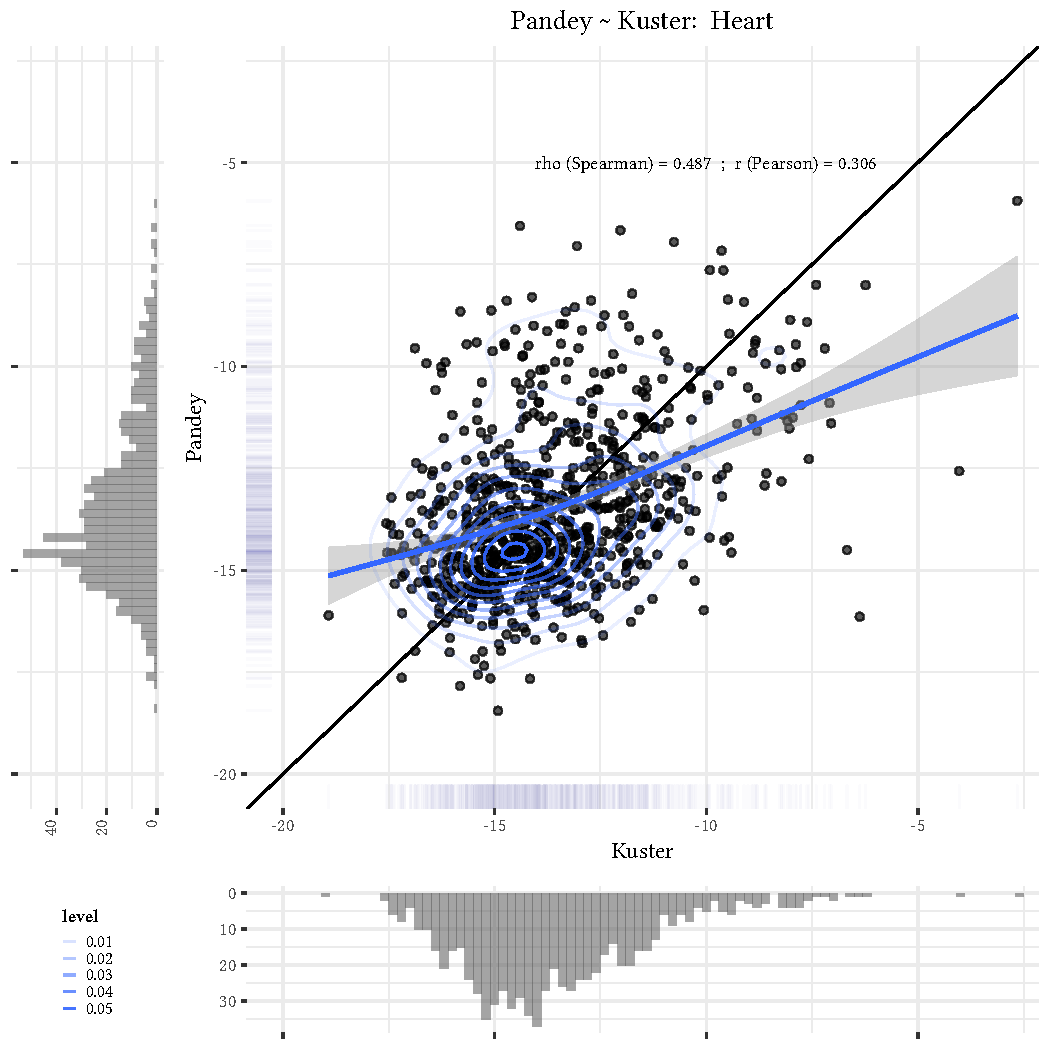
\includegraphics[scale=0.7]{proteomics/scatterplot/3D/heartKusterPandey.pdf}\centering
    \caption[Heart: Kuster vs Pandey]{\label{fig:scat3DheartKusterPandey}\textbf{%
    Scatterplot of Heart for Kuster and Pandey data.}
    The dispersion of expression is more significant than between \pandey\ and \cutler\
    (see \Cref{fig:scat3DheartCutlerPandey}).
    It is rather difficult to assess the protein expression in \Heart\ from
    \pandey\ (or \kuster) based on the other study.
    {\small The black line $y=x$ is only present as a visual reference.}}
\end{figure}

\begin{figure}[!htpb]
    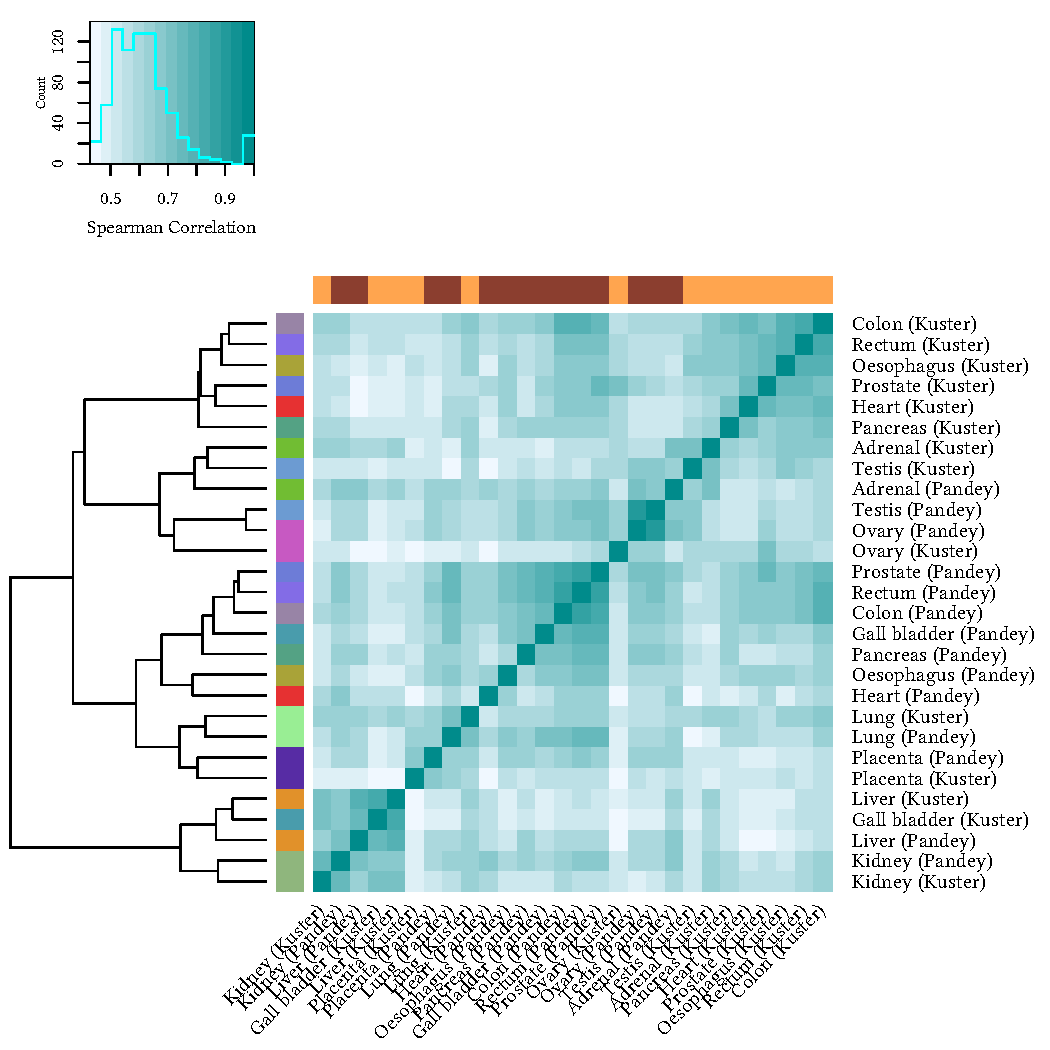
\includegraphics[scale=0.95]{proteomics/heatmap2DproteinSpearmanT14.pdf}\centering
    \caption[Heatmap of the 14 common tissues between Pandey and Kuster datasets
    (Spearman correlation)]{\label{fig:prot2DheatmapT14}\textbf{Heatmap of
    the fourteen common tissues between Pandey and Kuster datasets}
    based on the pairwise \textbf{Spearman correlations} of the expression levels of
    their 4,172 common proteins.
    \Placenta, \Lung\ and \Kidney\ \treps\ between \pandey\ and \kuster\ show
    an overall higher biological similarity than technical variability
    to the other tissues from the same study source.
    See also \Cref{fig:prot2DheatmapPearson,fig:scat2DPlacentaKusterPandey,fig:scat2DAdrenalPancreasKuster,fig:scat2DAdrenalPandeyPancreasKuster}.}
\end{figure}


\begin{figure}[!htpb]
    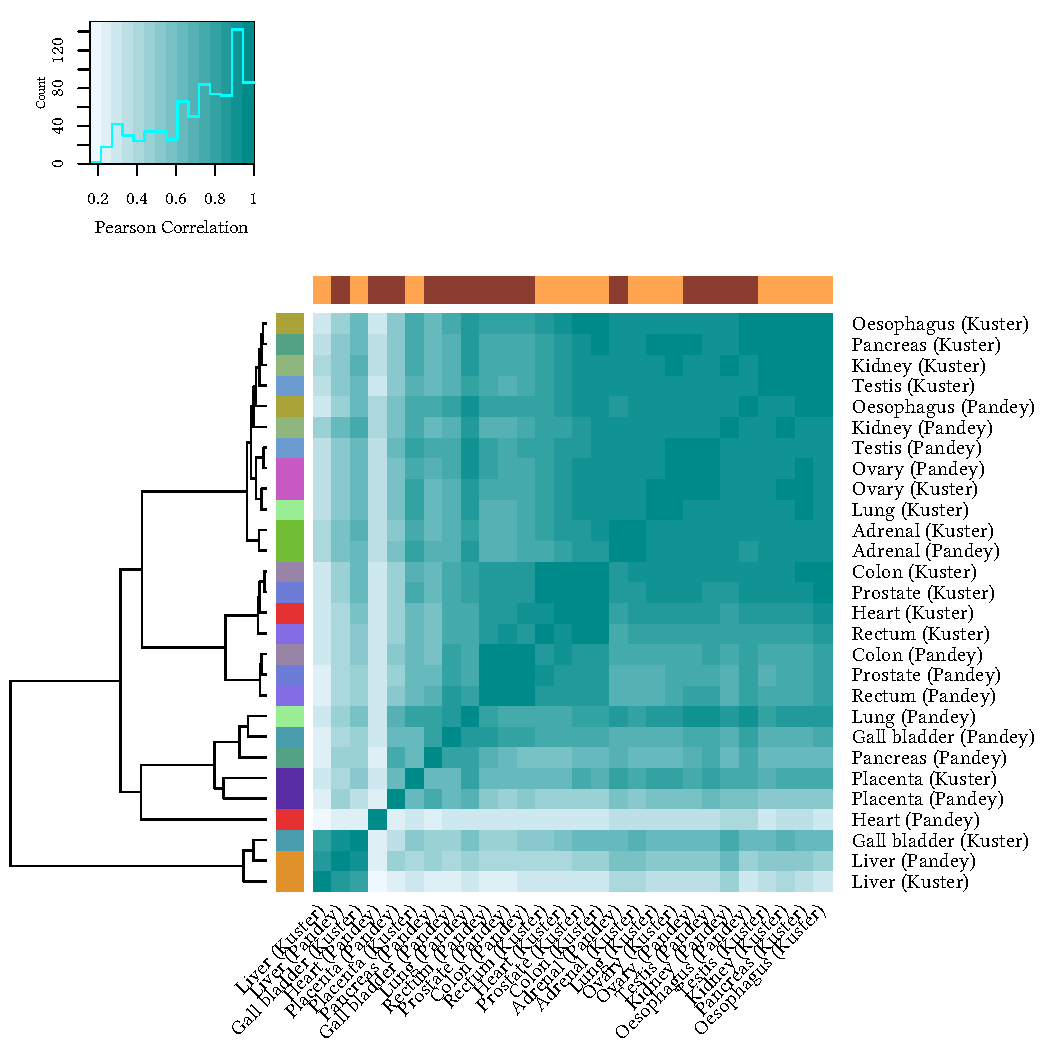
\includegraphics[scale=0.9]{proteomics/heatmap2DproteinPearsonT14.pdf}\centering
    \caption[Heatmap of the 14 common tissues between Pandey and Kuster
    datasets (Pearson correlation)]{\label{fig:prot2DheatmapPearson}\textbf{Heatmap
    of the fourteen common tissues between Pandey and Kuster datasets}
    based on the pairwise \textbf{Pearson correlations} of the expression levels of
    their 4,172 common proteins.
    Only \Placenta\ and \Adrenal\ \treps\ between \pandey\ and \kuster\ show
    a greater biological similarity than technical one.
    See also \Cref{fig:prot2DheatmapT14,fig:scat2DPlacentaKusterPandey,fig:scat2DAdrenalPancreasKuster,fig:scat2DAdrenalPandeyPancreasKuster}.}
\end{figure}

\begin{figure}[!htpb]
    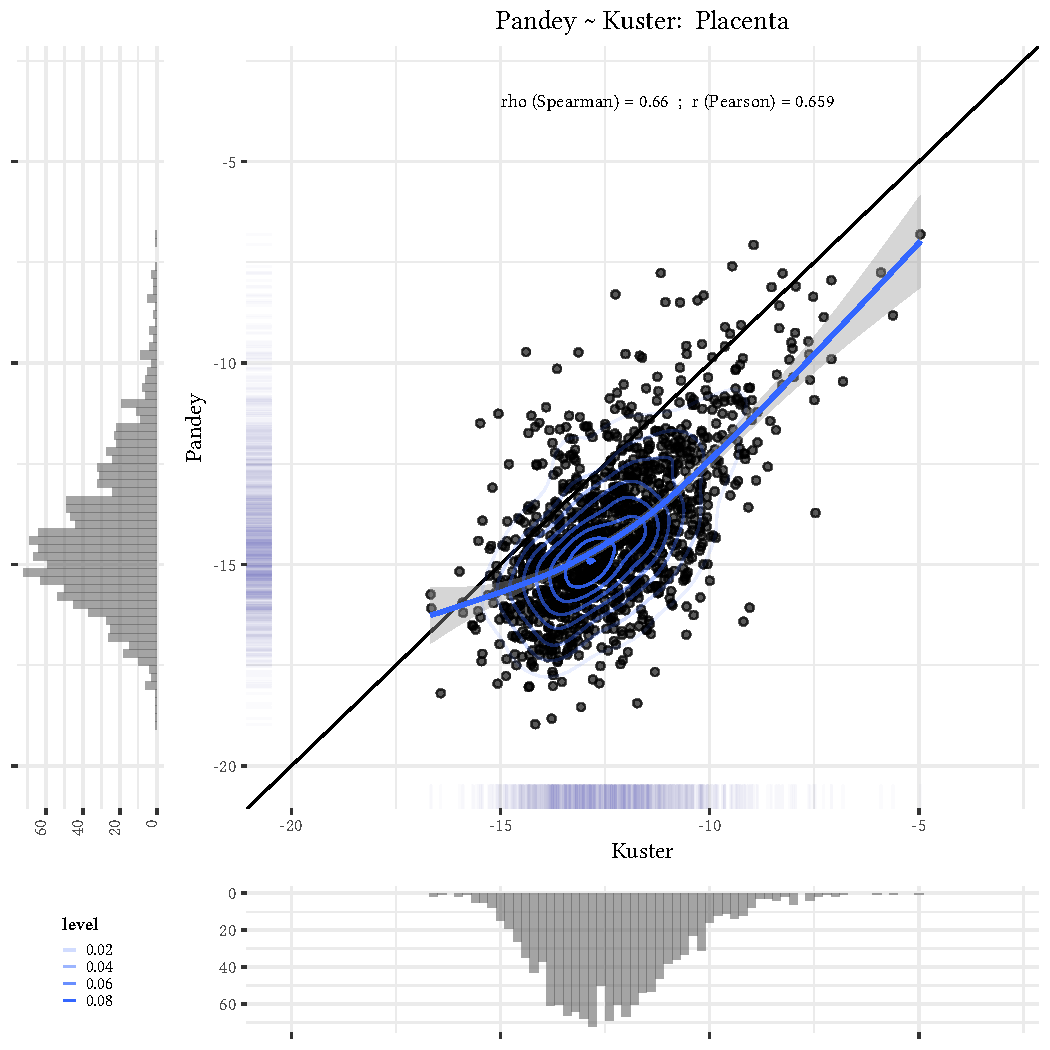
\includegraphics[scale=0.7]{proteomics/scatterplot/2D/PlacentaKusterPandey.pdf}\centering
    \caption[Placenta: Kuster vs Pandey]{\label{fig:scat2DPlacentaKusterPandey}\textbf{%
    Scatterplot of Placenta for Kuster and Pandey data.}
    While the expression of some proteins are more spread between both datasets,
    there is an overall strong linear correlation between \pandey\ and \kuster\
    for their \placenta\ tissue.
    Besides a few exception,
    protein expression levels in \pandey\ seem to be underestimated compared to
    \kuster.
    This is most probably due to the normalisation method.
    {\small The black line $y=x$ is only present as a visual reference.}}
\end{figure}

\begin{figure}[!htpb]
    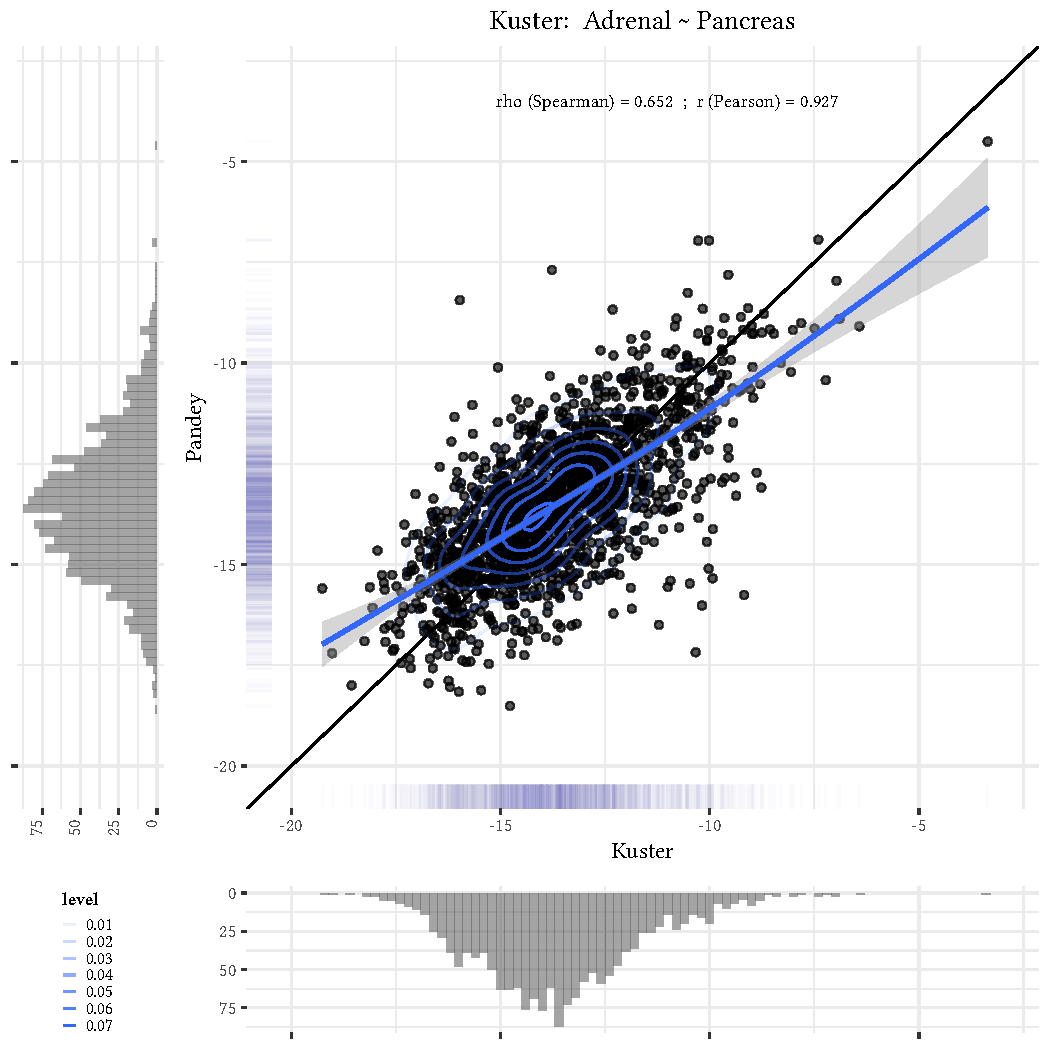
\includegraphics[scale=0.7]{proteomics/scatterplot/2D/PancreasAdrenalKuster.pdf}\centering
    \caption[Kuster: Pancreas vs Adrenal]{\label{fig:scat2DAdrenalPancreasKuster}\textbf{%
    Scatterplot of Pancreas and Adrenal (from Kuster).}
    Although Kuster's \Pancreas\ and \Adrenal\ are never found
    in \Cref{fig:prot2DheatmapT14,fig:prot2DheatmapPearson}
    as the most similar to each other,
    their expression levels present a strong linear relationship to each other.
    The dispersion and outliers seem insuffisant
    to unquestionably distinguish different tissues.
    \Cref{fig:scat2DAdrenalPandeyPancreasKuster} is even more compelling.
    {\small The black line $y=x$ is only present as a visual reference.}}
\end{figure}


\begin{figure}[!htpb]
    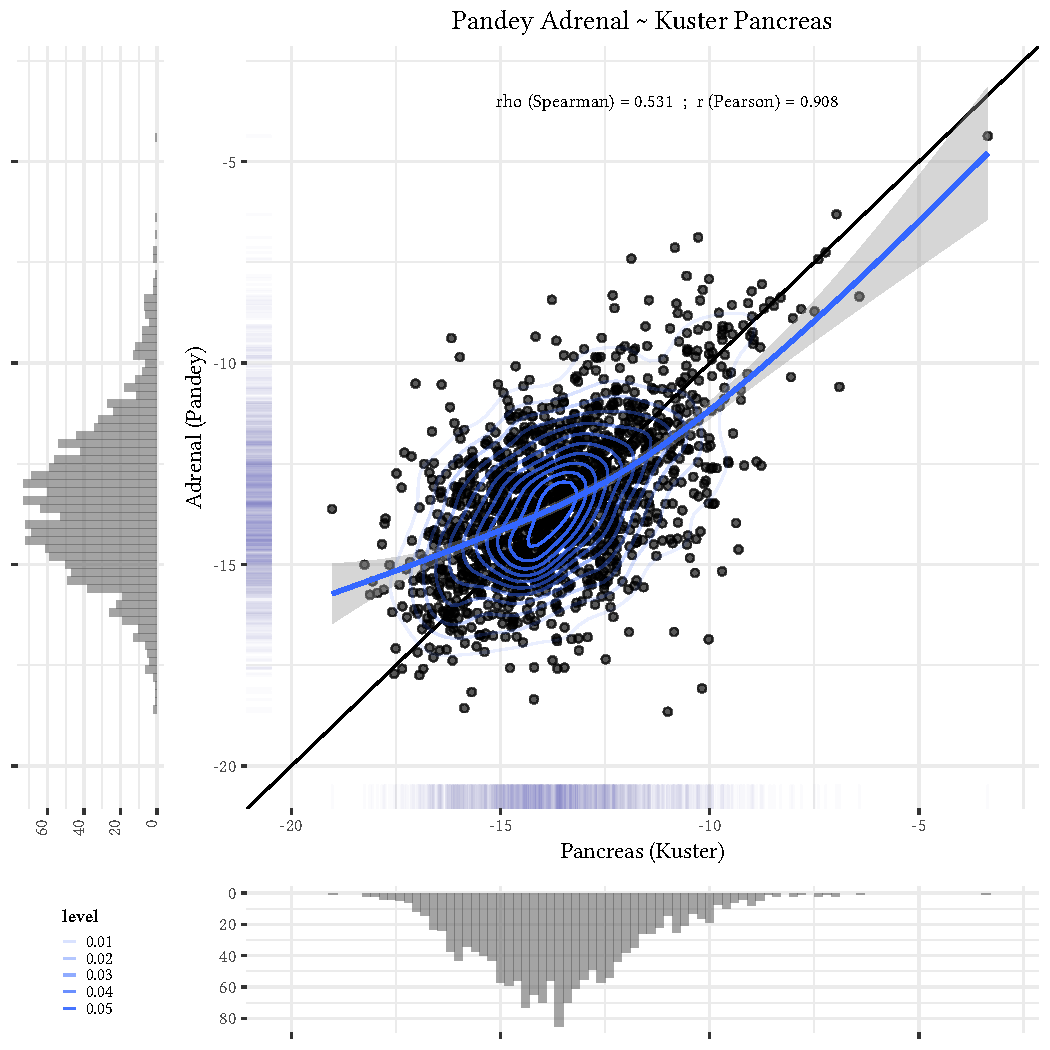
\includegraphics[scale=0.7]{proteomics/scatterplot/2D/PancreasKusterAdrenalPandey.pdf}\centering
    \caption[Kuster Pancreas vs Pandey Adrenal]{\label{fig:scat2DAdrenalPandeyPancreasKuster}\textbf{%
    Scatterplot of Kuster Pancreas and Pandey Adrenal.}
    As in \Cref{fig:scat2DAdrenalPancreasKuster},
    Kuster's \pancreas\ and Pandey's \adrenal\ are never found as the most similar
    to each other.
    Once again,
    there is a strong linear relationship between their protein expression levels,
    even though the dispersion is greater and the outliers more numerous.
    {\small The black line $y=x$ is only present as a visual reference.}}
\end{figure}


\begin{figure}[!htpb]
    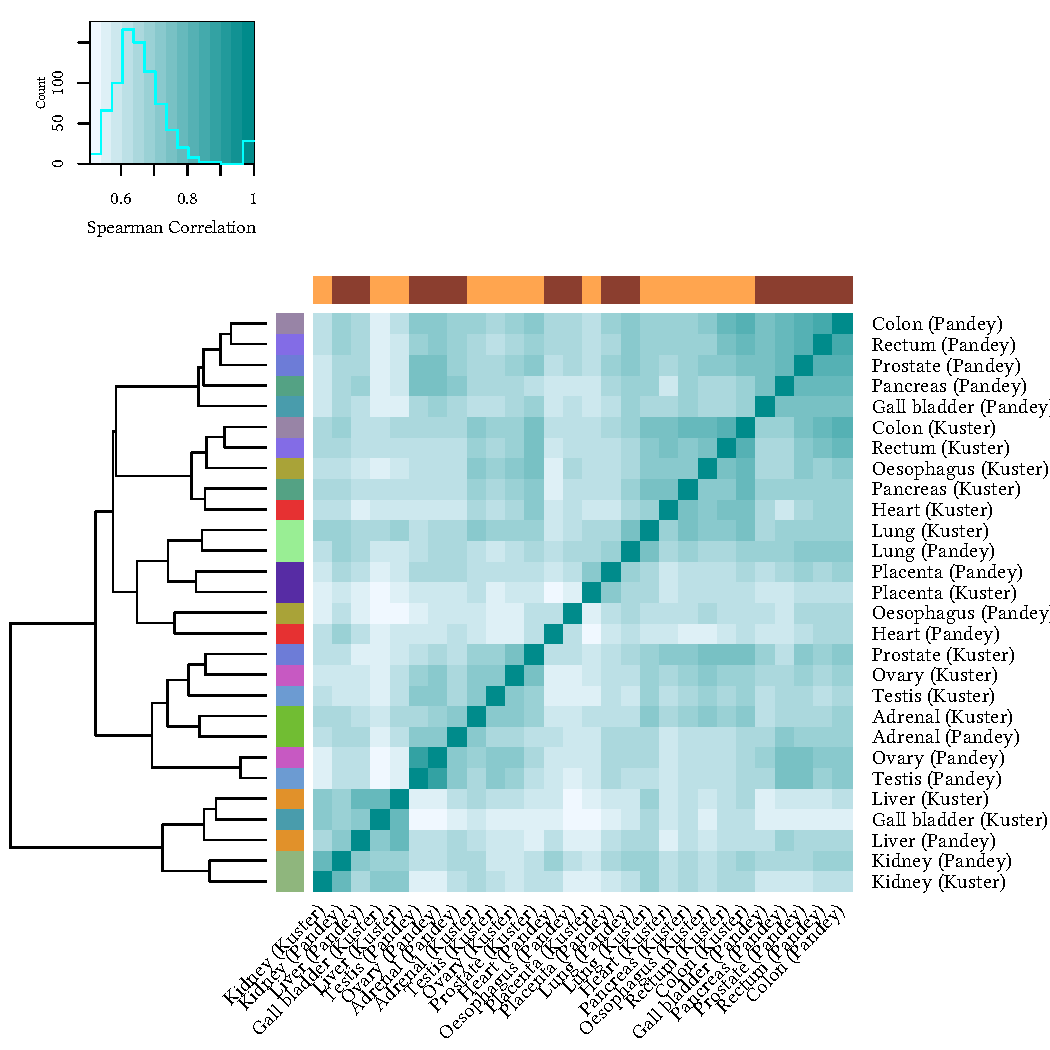
\includegraphics[scale=0.9]{proteomics/heatmap2DproteinSpearmanT14_PPKM.pdf}\centering
    \caption[Heatmap of the 14 common tissues between Pandey and Kuster
    (Spearman correlation --- PPKM)]{\label{fig:heatmap3DProtT14PPKM}\textbf{Heatmap
    of the fourteen common tissues between Pandey and Kuster (PPKM) datasets}
    based on the pairwise Spearman correlations of the expression levels of
    their 8,680 common proteins.
    Compared to \Cref{fig:prot2DheatmapT14},
    once again \Placenta, \Lung, \Kidney\ are displaying a higher biological signal
    than technical variability.
    This is also the case of \Adrenal\ tissue (as in \Cref{fig:prot2DheatmapPearson}).
    Thus, the results are similar to the ones from the first quantification method.}
\end{figure}
